\documentclass[11pt,letter]{article}
\usepackage{graphicx}
\usepackage{pdflscape}
\usepackage{geometry}
\setlength{\textheight}{7.5in}
\setlength{\oddsidemargin}{.125in}
\setlength{\textwidth}{6.25in}
\begin{document}
\begin{center}
SUMMER 2015 CSCI 3308 PROJECT PROPOSAL
\end{center}
\begin{enumerate}
\item \textbf{Project Members}: Joseph Bundrant, Joseph Jackson, Daniel Velasco, Dylan Nguyen
\item \textbf{Title}: Let's find a ... (Letsfinda...)
\item Description: A website aimed towards providing users with deals and hotspots for pubs or restaurants based on a given location and date.
\item \textbf{Vision Statement}: A singular gateway to finding good deals and popular adult beverage establishments
\item \textbf{Motivation}: While services such as Google maps offer an idea of what establishments are in an area and others such as Groupon provide special deals, it can sometimes be tedious having to search and switch between the two (or even three if you start considering major review sites). Thus, we would like to create a singular gateway for users to find a place and get all the available information such as deals and rating in one place.
\item \textbf{Risks}: Overall the group has little experience working with JavaScript, PHP, and APIs.
\begin{enumerate}
\item \textbf{Mitigation Strategy}: We intend to divide the project into sections based on the language knowledge required, so that members are not required to learn all 3 facets and can focus on a single area.
\end{enumerate}
\item \textbf{VCS}: Github Link: https://github.com/dyng9409/letsfinda
\item \textbf{List of requirements}

\begin{center}
\begin{tabular}{|c|p{0.65\linewidth}|c|}
\hline
\multicolumn{3}{|l|}{\textbf{User Requirements}} \\
\hline
\textbf{ID} & \textbf{Description} & \textbf{Agile Sizing} \\
\hline
USER-01 & As a user, I want to be able to specify a date and location, so that I can accurately find locations of interest& 2 \\
\hline
USER-02 & As a user, I want to be able to visually see the location hits, so that I can better gauge their proximity & 8 \\
\hline
USER-03 & As an admin, I want users to be able to report expired or incorrect deals, so that we can maintain accuracy & 5 \\
\hline
\end{tabular}
\end{center}

\begin{center}
\begin{tabular}{|c|p{0.65\linewidth}|c|}
\hline
\multicolumn{3}{|l|}{\textbf{Functional Requirements}} \\
\hline
\textbf{ID} & \textbf{Description} & \textbf{Agile Sizing}\\
\hline
FUNC-01 & Reporting an invalid or expired deal should have a captcha and comment box to prevent spam & 3 \\
\hline
\end{tabular}
\end{center}

\begin{center}
\begin{tabular}{|c|p{0.65\linewidth}|c|}
\hline
\multicolumn{3}{|l|}{\textbf{Non-functional Requirements}} \\
\hline
\textbf{ID} & \textbf{Description} & \textbf{Agile Sizing} \\
\hline
NONF-01 & Results should take no more than 5-6 seconds to load & 1 \\
\hline
NONF-02 & Search query should be able to expand to more/different services & 8 \\
\hline
\end{tabular}
\end{center}
\item Methodology: Agile 
\item Project Tracking Software: Trello
\item Project Plan 
\pagebreak

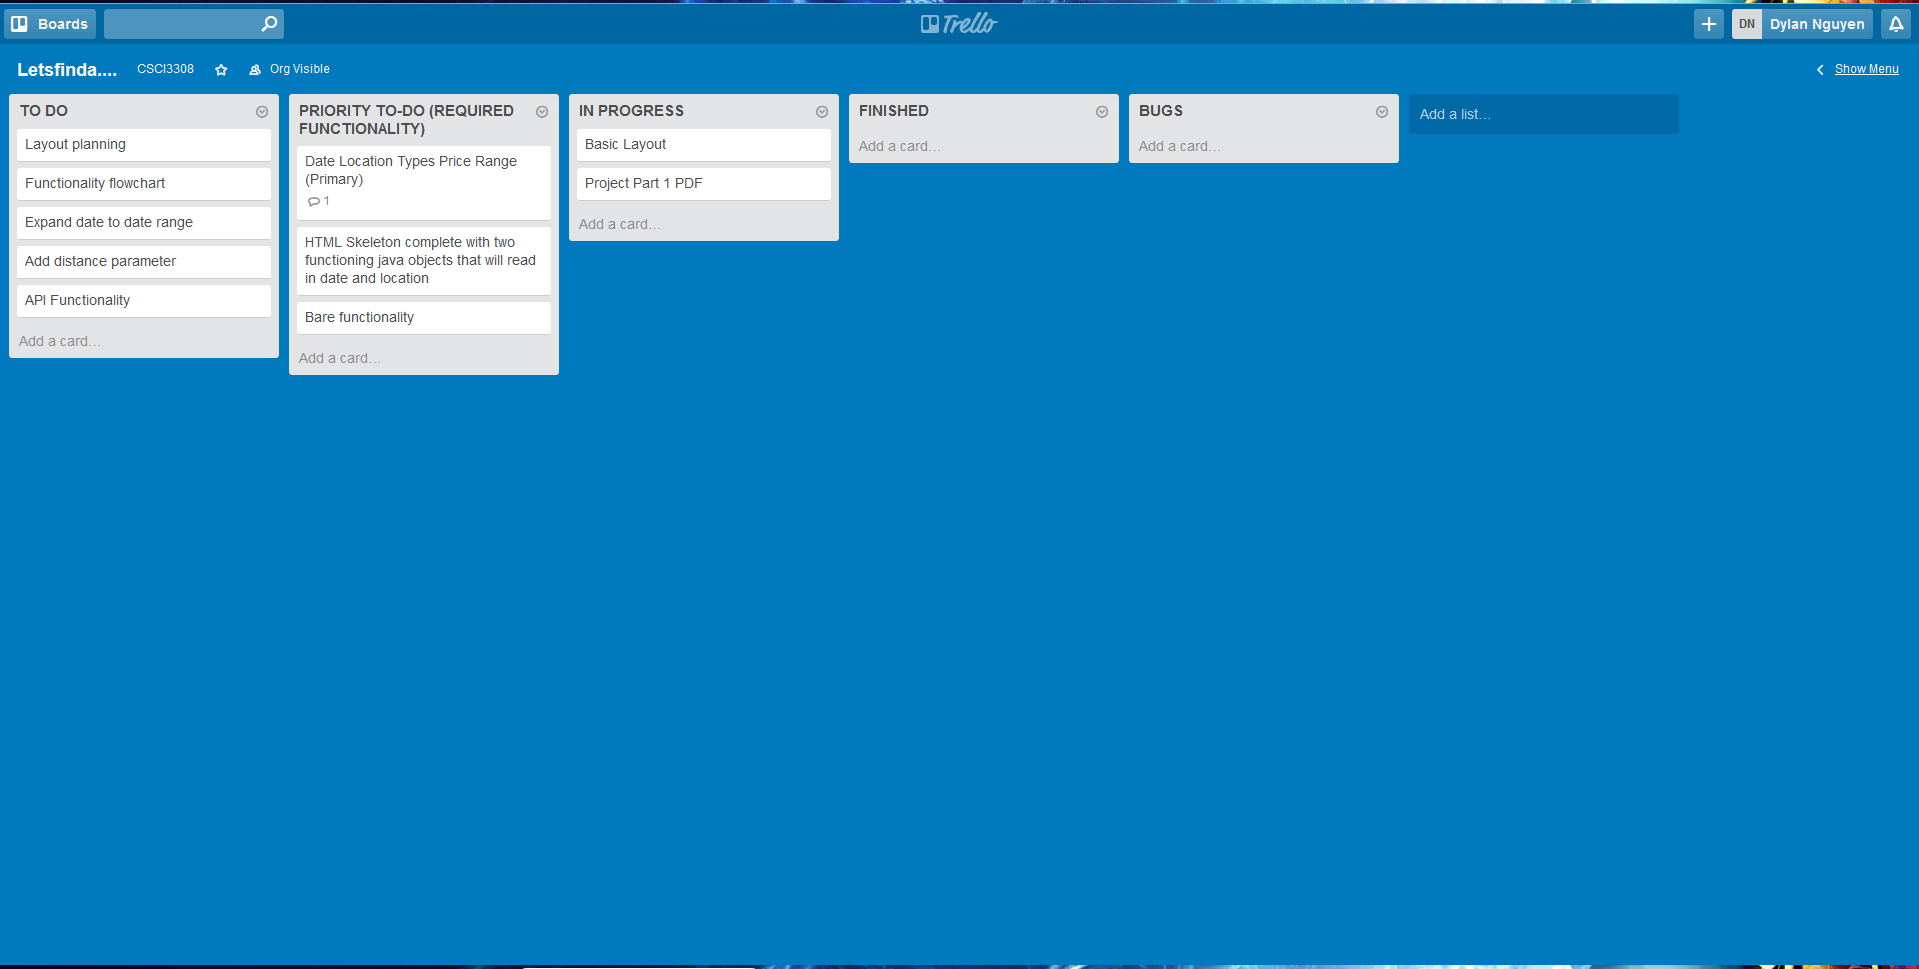
\includegraphics[scale = 0.4, angle = 90]{plan.jpg}

\pagebreak

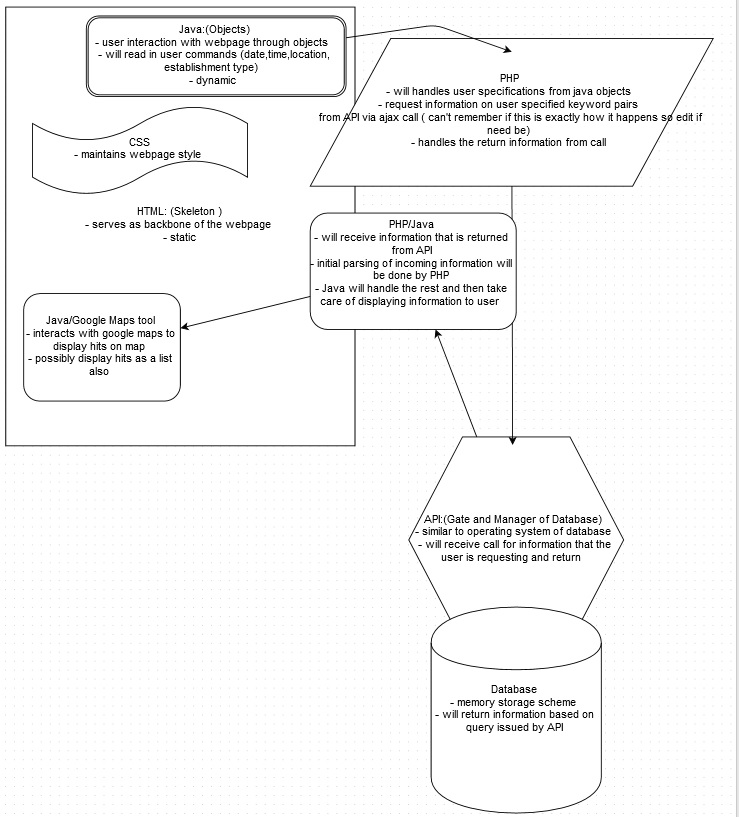
\includegraphics[scale=0.7]{flow.jpg}

\end{enumerate}
\end{document}